\subsection{Использование АР для детектирования ШПС}

\subsection{Алгоритм обнаружения ШПС с использованием процедуры БПФ}

Точность АР метода напрямую зависит от точности оценки АКФ гармонического сигнала. Основным способом повышения точности оценки АКФ является увеличение размера выборки,
что в случае модулированного сигнала может быть затруднительным.В данной работе предлагается использовать алгоритм увеличения ОСШ мектодом последовательного вычисления
АКФ \cite{ostanin_akf}. Для снижения вычислительных затрат указанный алгоритм предлагается реализовывать с использованием процедуры БПФ. 
Введем следующие обозначения: ${x}$ – вектор входного сигнала после снятия ПСП, ${F}$ – матрица прямого преобразования Фурье, ${F^{-1}}$- матрица обратного преобразования Фурье.
Оценку АКФ на первом шаге можно получить следующим образом:

\begin{center}
\begin{equation}
	\label{eq:akf_1}
	\hat{r_1} = F^{-1}\left[ Fx \cdot (Fx)^* \right] = F^{-1} \left[ \left| Fx \right| ^2 \right]
\end{equation}
\end{center}

Здесь знак ${(\cdot)}$  означает поэлементное перемножение векторов, ${\left| Fx \right| ^2}$ - поэлементное возведение модуля комплексного числа в квадрат, ${*}$ - означает
комплексное сопряжение.  Следуя алгоритму, изложенному в \cite{ostanin_akf} вычислим оценку АКФ от ${\hat{r_1}}$:

\begin{center}
\begin{eqnarray}
	\label{eq:akf_2}
	\hat{r_2} & = & F^{-1}\left[ F \hat{r_1} \cdot (F \hat{r_1})^* \right] = \nonumber \\
		& = & F^{-1}	\left[ 
				FF^{-1} \left[
						\left| Fx \right| ^2
					\right]
						\cdot \left( FF^{-1} \left[ \left| Fx \right| ^2 \right]
					\right) ^*
			\right] = \nonumber \\
		& = & F^{-1} \left[ \left| Fx \right| ^2 \cdot \left[ \left| Fx \right| ^2 \right] ^* \right] =  \nonumber \\
		& = & F^{-1} \left[ \left| Fx \right| ^4 \right]
\end{eqnarray}
\end{center}

Рассуждая аналогично, можно показать, что уточненная оценка АКФ на K-ом шаге алгоритма, рассмотренного в \cite{ostanin_akf}
может быть получена без использования итераций с помощью выражения:

\begin{center}
\begin{equation}
	\label{eq:akf_3}
	\hat{r_K} = F^{-1}\left[ \left| Fx \right| ^{2^K} \right]
\end{equation}
\end{center}

Схематически алгоритм получения уточненной оценки АКФ на третьем шаге представлен на рисунке \ref{pic:akf_pic}.

\begin{figure}[H]
	\center\scalebox{0.8}{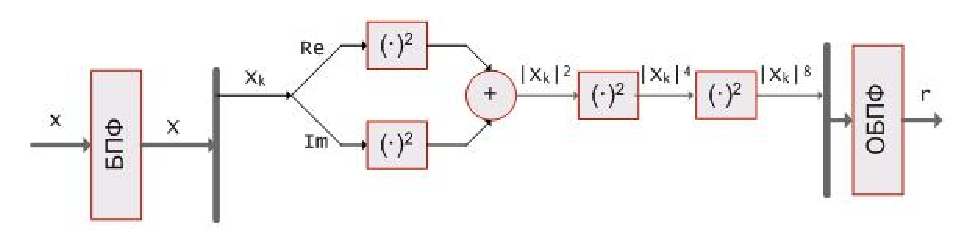
\includegraphics[width=1\linewidth]{akf_fft.eps}}
	\caption{Усовершенствованный итеративный алгоритм получения АКФ}
	\label{pic:akf_pic}
\end{figure}


\subsection{Алгоритм уточнения оценки АКФ гармонического сигнала}
\subsection{Алгоритм обнаружения и оценки параметров ШПС в условиях интерференции (DMA + уточненный АР)}
\subsection{Результаты численного моделирования}
\subsection{Результаты обработки сигнала GPS}

\subsection*{Выводы}

\newpage
